%%%%%%%%%%%%%%%%%%%%%%%%%%%%%%%%%%%%%%%%%%%%%%
%                insertmeeting
% 1) Title (something creative & funny?)
% 2) Date (MM/DD/YYYY)
% 3) Location (ex. Hagerty High School)
% 4) People/Committees Present 
% 5) Picture 
% 6) Start Time & Stop Time (ex. 12:30AM to 4:30PM)
%%%%%%%%%%%%%%%%%%%%%%%%%%%%%%%%%%%%%%%%%%%%%%
\insertmeeting 
	{Meeting Example} 
	{11/08/21}
	{Hagerty High School}
	{Nathan, Ritam}
	{Images/RobotPics/robot.jpg}
	{2:30 - 4:30}
	
\hhscommittee{Hardware}
\noindent\hfil\rule{\textwidth}{.4pt}\hfil
\subsubsection*{Goals}
\begin{itemize}
    \item CAD and assemble arm holder
    \item Ensure robot fits within 18
    \item Make sure hardware is complete so software can start working on autonomous
 

\end{itemize} 

\noindent\hfil\rule{\textwidth}{.4pt}\hfil

\subsubsection*{Accomplishments}
Referring to our sketch of the arm holder that we made during the last meeting, we got onto onshape and started creating the part. The main thing we needed to build was the hinge part, which would allow the holder to spin freely upwards when the arm moved out of the way.we created the hinge to connect onto the side of the rev extrusions that support the arm. The hinge hole was made 3.5 millimeters wide to let us use an M3 screw as the shaft for the holder (Figure \ref{fig:pic1}). All of this will make assembly very easy and will allow us to change the starting angle of the arm by simply sliding the holder up or down on the extrusion. We started printing the hinge while we created the holder. The holder was designed as an l shaped part we plan on laser cutting. It has a hole on one end of the l for a rubber band or piece of surgical tubing to be threaded through, which will provide the tension necessary to move the holder out of the way when the arm lifts up. Once all of the parts were cut and printed, we put them onto the robot. When we tested out the mechanism, we found that it worked perfectly (Figure \ref{fig:pic2} and Figure \ref{fig:pic3}). Finding that it functioned as we wanted it to, we moved the robot onto the sizing cube, adjusted the height of the holder to support the arm at the right angle and found that the robot fit within 18 inches (Figure \ref{fig:pic4}). With that, all of the hardware elements we wanted to put onto the robot before the first meet were complete, and it is time for software to take the reins and start creating auto!

 

\begin{figure}[ht]
\centering
\begin{minipage}[b]{.48\textwidth}
  \centering
  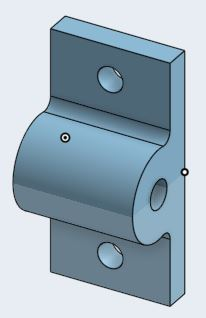
\includegraphics[width=0.95\textwidth]{Meetings/November/11-08-21/11-8-21_Hardware_Figure1 - Nathan Forrer.JPG}
  \caption{The M3 Screw Holder}
  \label{fig:pic1}
\end{minipage}%
\hfill%
\begin{minipage}[b]{.48\textwidth}
  \centering
  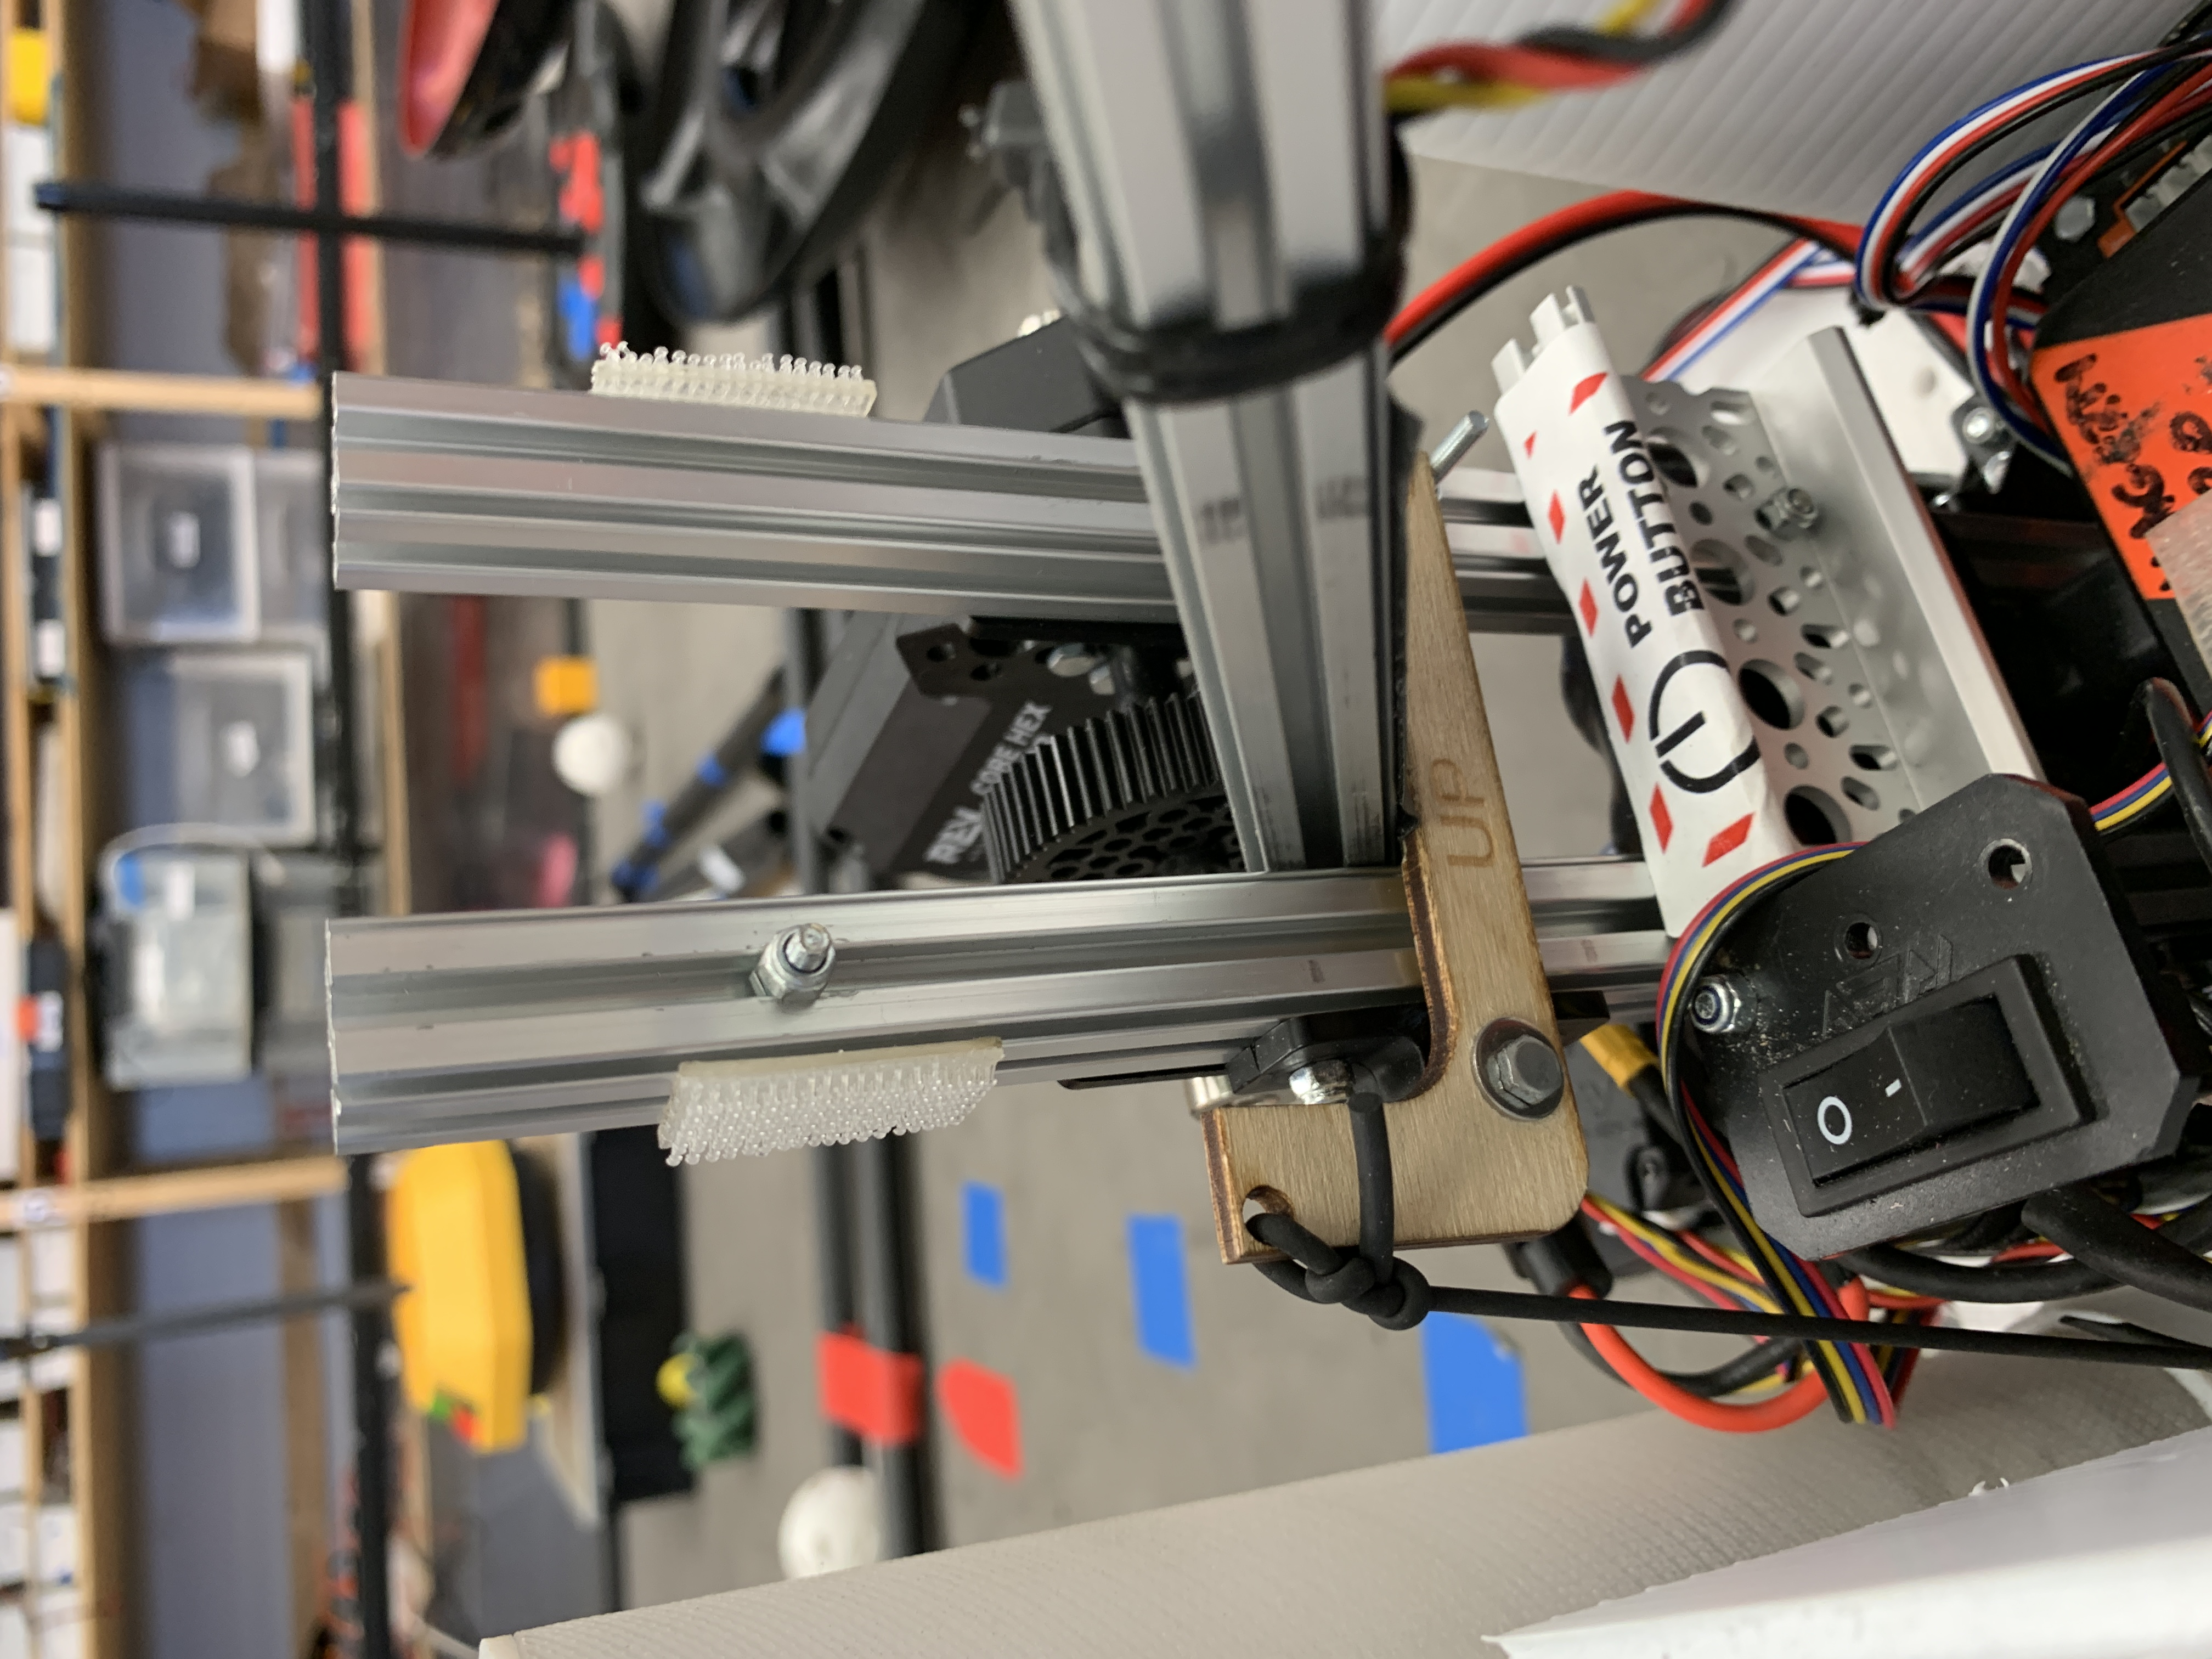
\includegraphics[width=0.95\textwidth]{Meetings/November/11-08-21/11-8-21_Hardware_Figure2 - Nathan Forrer.JPG}
  \caption{The arm resting on the holder}
  \label{fig:pic2}
\end{minipage}
\end{figure}

\begin{figure}[ht]
\centering
\begin{minipage}[b]{.48\textwidth}
  \centering
  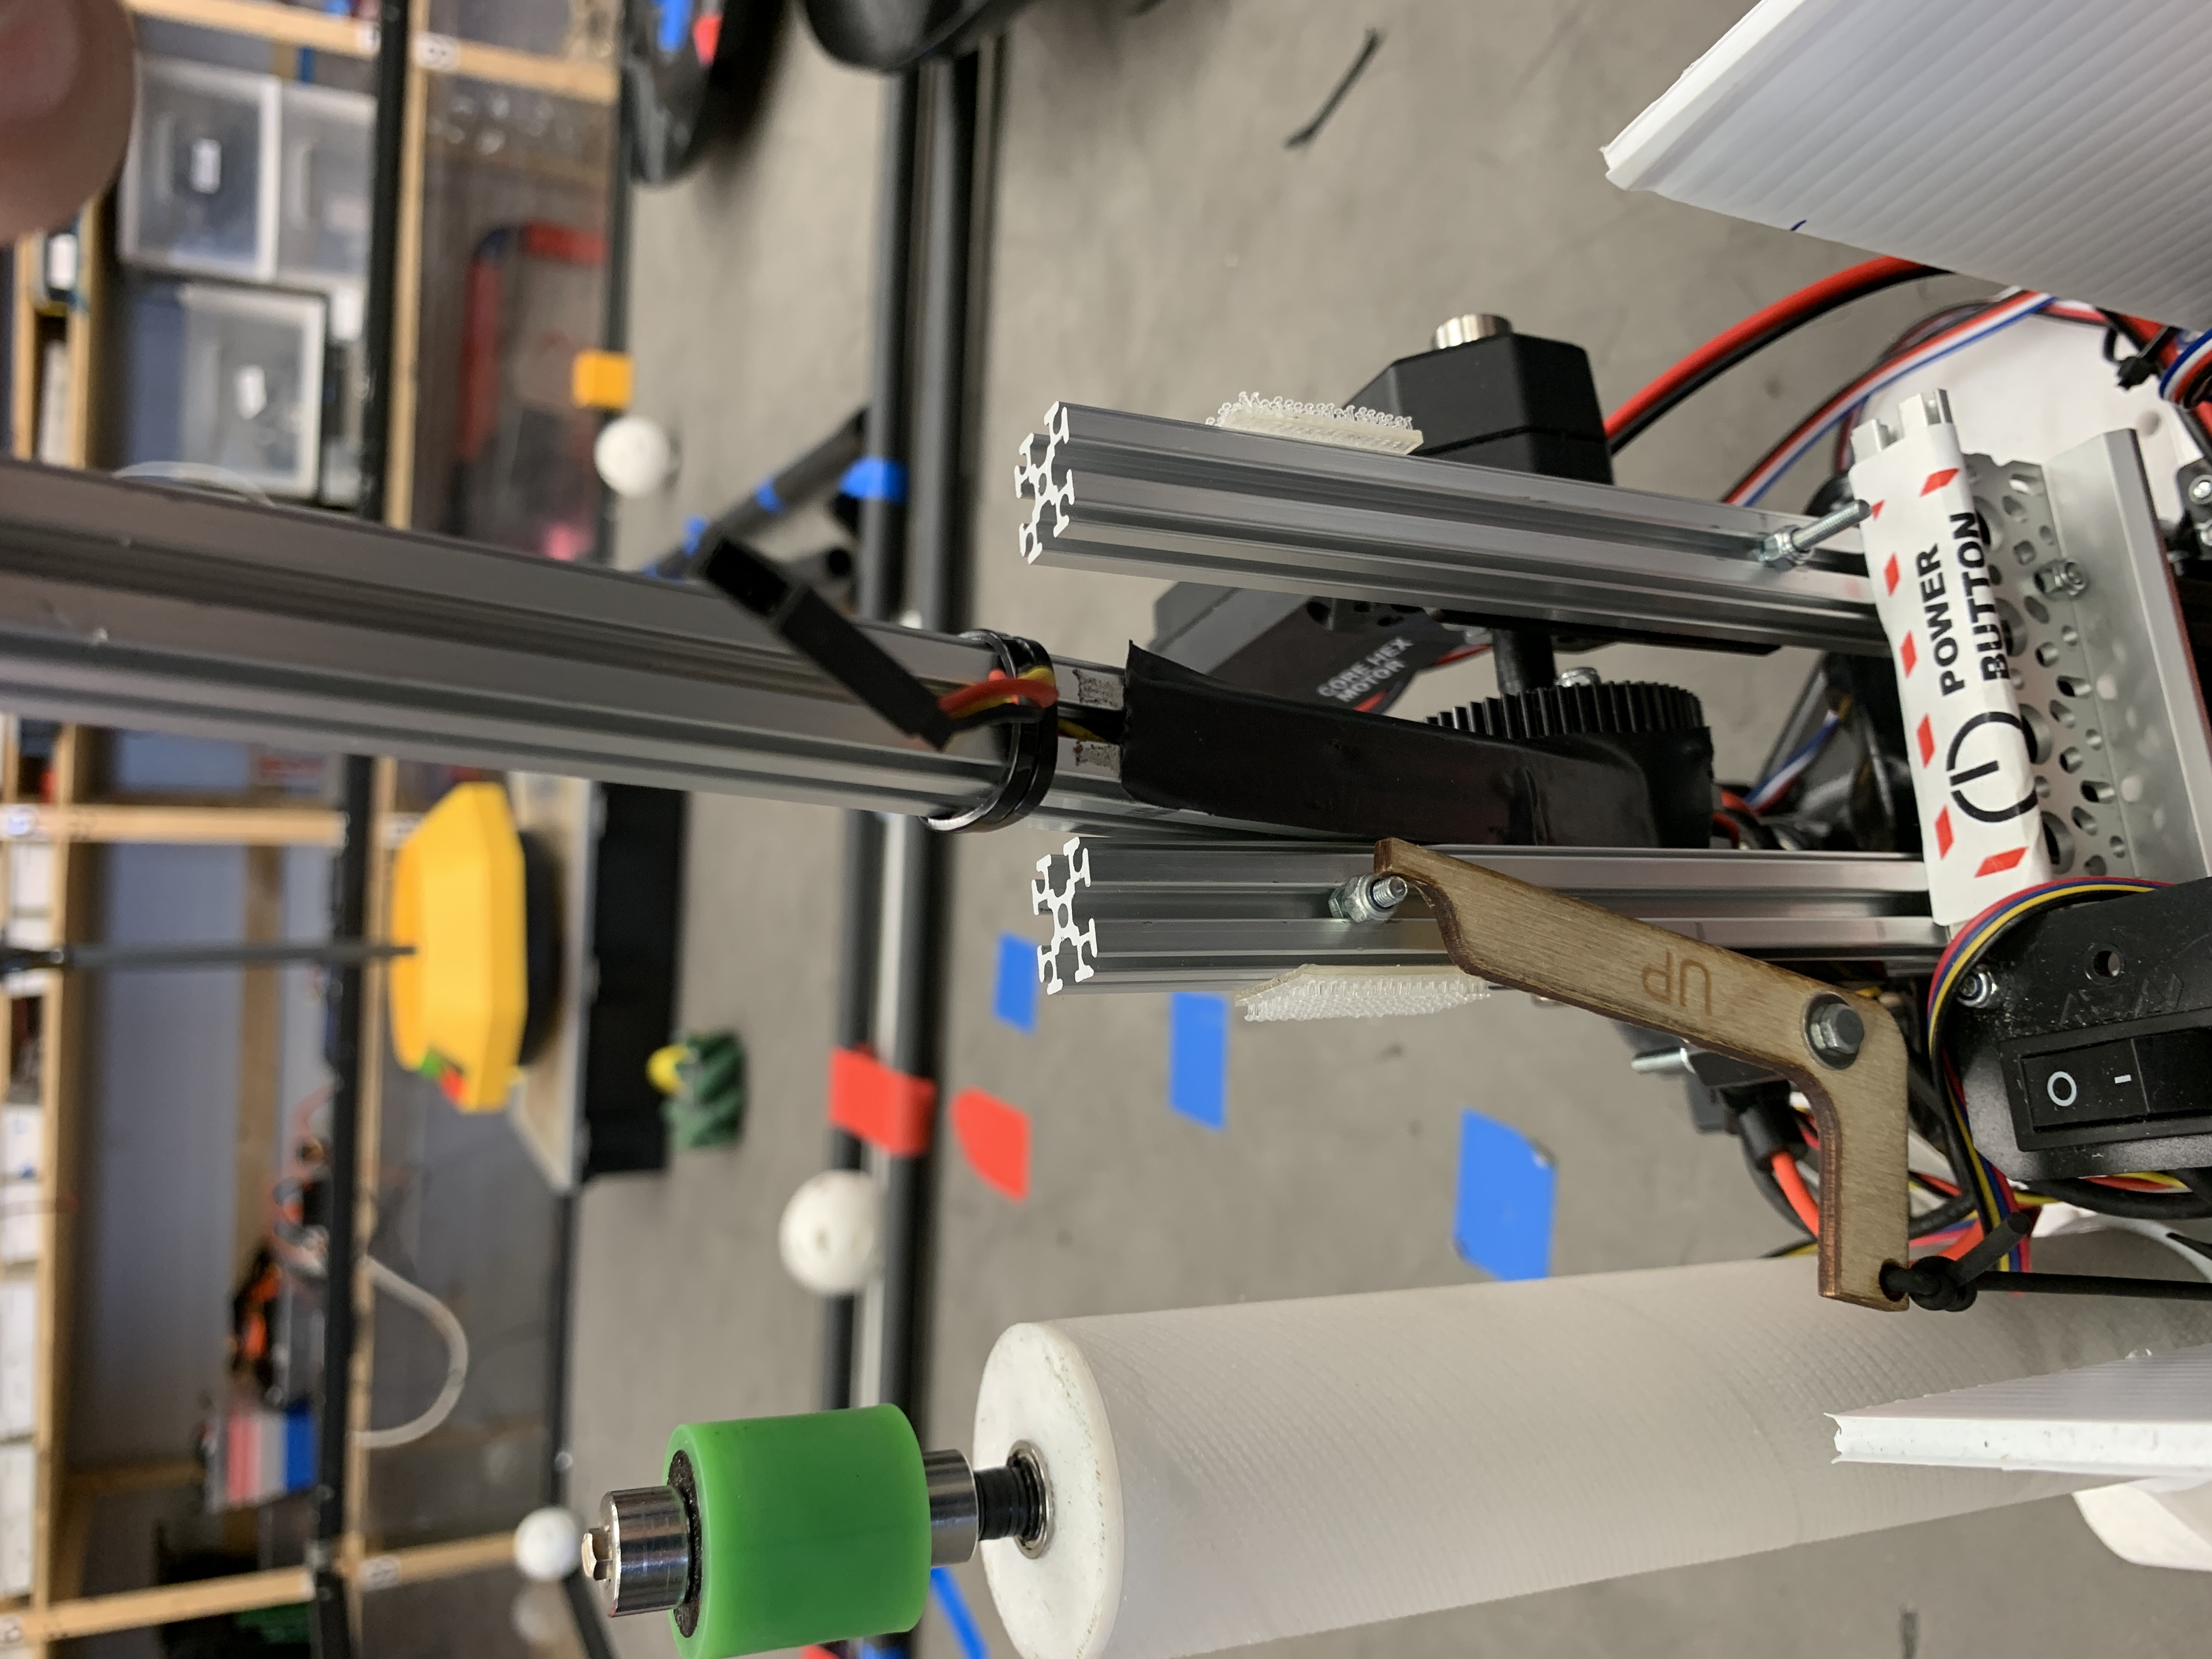
\includegraphics[width=0.95\textwidth]{Meetings/November/11-08-21/11-8-21_Hardware_Figure3 - Nathan Forrer.JPG}
  \caption{The holder moves out of the way}
  \label{fig:pic3}
\end{minipage}%
\hfill%
\begin{minipage}[b]{.48\textwidth}
  \centering
  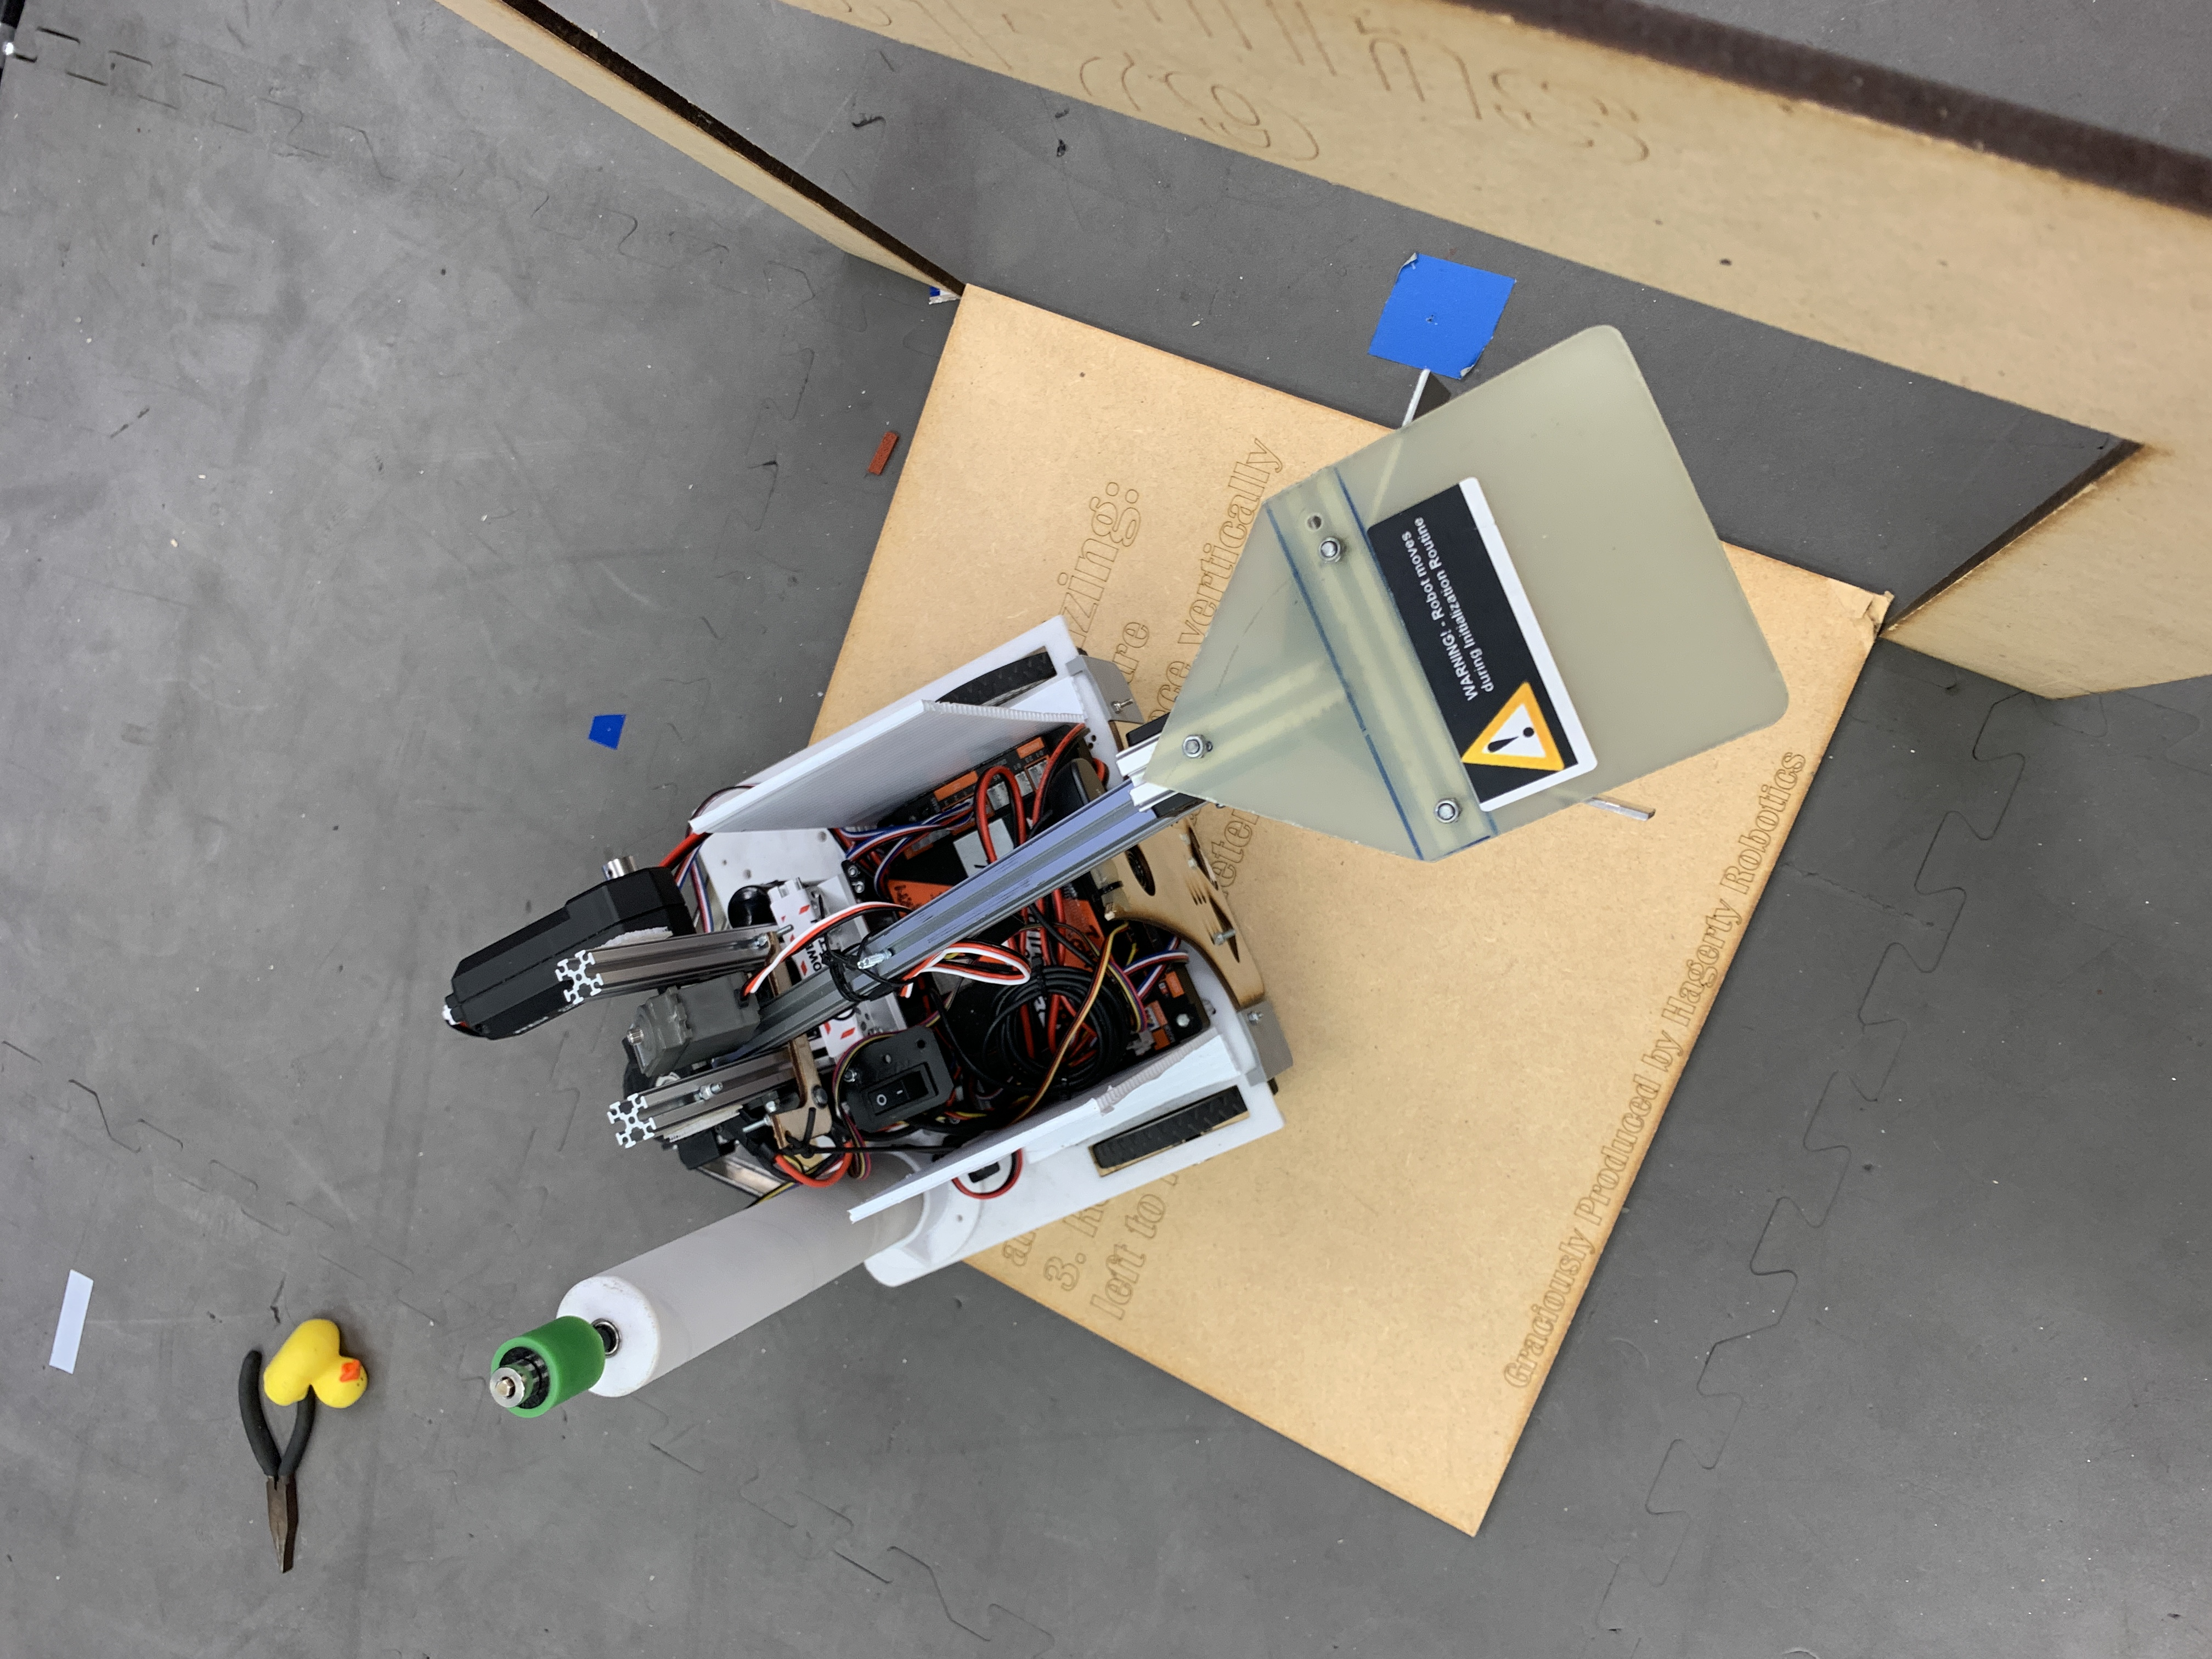
\includegraphics[width=0.95\textwidth]{Meetings/November/11-08-21/11-8-21_Hardware_Figure4 - Nathan Forrer.JPG}
  \caption{Robot fitting in the sizing}
  \label{fig:pic4}
\end{minipage}
\end{figure}


\whatsnext{
\begin{itemize}
    \item Let software create the autonomous program
    \item Be ready to fix any problems that come up.

\end{itemize} 
}

